%% ----------------------------------------------------------------
%% PACKAGES
%% ----------------------------------------------------------------
\documentclass[titlepage, 12pt]{article}
\usepackage[table, xcdraw, dvipsnames]{xcolor}
\usepackage[utf8]{inputenc}
\usepackage[spanish]{babel}
\usepackage{amsmath}
\usepackage{booktabs}
\usepackage[RPvoltages]{circuitikz}
\usepackage{enumitem}
\usepackage{fancyhdr}
\usepackage{float}
\usepackage{geometry}
\usepackage{graphicx}
\usepackage[hidelinks]{hyperref}
\usepackage{lastpage}
\usepackage{pdflscape}
\usepackage{parskip}
\usepackage{siunitx}
\usepackage{subcaption}
\usepackage{tabularx}
\usepackage{tikz}
\usepackage{xfrac}


%% ----------------------------------------------------------------
%% SETTINGS
%% ----------------------------------------------------------------
\decimalpoint
\geometry{
  a4paper,
  total={170mm,247mm},   %210x297mm
  left=20mm,
  top=20mm,
}
\renewcommand{\tablename}{Tabla}
\newcommand{\fecha}{16/08/2021} % #FIXME
\newcommand{\version}{1.0}


%% ----------------------------------------------------------------
%% HEADER/FOOTER
%% ----------------------------------------------------------------
\pagestyle{fancy}
\fancyhf{}
\lhead{Calibrador y caracterizador de sondas de corriente}
\rhead{Especificación funcional}
\lfoot{Fecha: \fecha}
\cfoot{Versión \version}
\rfoot{Página \thepage \hspace{1pt} de \pageref{LastPage}}

\setlength{\headheight}{30pt}


%% ----------------------------------------------------------------
%% TITLE
%% ----------------------------------------------------------------
\title{Especificación funcional:\\Calibrador y caracterizador de sondas de corriente}
\author{Agustín Aon Sanchez\\
Facultad de Ingeniería\\
Universidad Nacional de Mar del Plata}
\date{Versión \version}


%% ----------------------------------------------------------------
%% BEGIN
%% ----------------------------------------------------------------
\begin{document}
\maketitle


%% ----------------------------------------------------------------
%% DOCUMENT
%% ----------------------------------------------------------------

%% ----------------------------------------------------------------
\section{Ficha del documento}
%% ----------------------------------------------------------------
\begin{table}[!hbtp]
  \centering
  \begin{tabular}{|c|c|c|c|}
  \hline
  \rowcolor[HTML]{C0C0C0}
  Fecha  & Versión  & Descripción     & Autor               \\ \hline
  \fecha & \version & Versión inicial & Agustín Aon Sanchez \\ \hline
  \end{tabular}
\end{table}

\newpage
\tableofcontents
\newpage
\listoffigures
\newpage


%% ----------------------------------------------------------------
\section{Introducción}
%% ----------------------------------------------------------------
Este documento corresponde a la Especificación Funcional para el proyecto final titulado Calibrador y caracterizador de sondas de corriente. Esta especificación se ha estructurado basándose en la información mencionada en el documento Especificación de Requerimientos (ER) versión 3.0.

  %% ----------------------------------------------------------------
  \subsection{Propósito del documento}
  %% ----------------------------------------------------------------
  El presente documento tiene como propósito proveer información detallada de cómo funcionará la solución, cuáles serán sus comportamientos deseados y cómo se deberá construir, con base en los requerimientos anteriormente definidos en la ER.

  Esta especificación funciona está dirigida a aquellos encargados del desarrollo de este proyecto. Además, este documento puede servir de soporte a aquellas personas que en un futuro deseen realizar un dispositivo similar.

  %% ----------------------------------------------------------------
  \subsection{Alcance del proyecto}
  %% ----------------------------------------------------------------
  El proyecto abarca la definición de los requerimientos, la implementación de la solución y la presentación final de la misma.

  Los requerimientos fueron planteados junto con el Laboratorio de Instrumentación y Control (LIC) de la Facultad de Ingeniería de la Universidad Nacional de Mar del Plata. Es en este laboratorio donde se realizará la mayor parte de este proyecto, haciendo uso de los recursos disponibles, bajo la guía del director del proyecto.

  La implementación de la solución será también realizada en el LIC.

  %% ----------------------------------------------------------------
  \subsection{Personal involucrado}
  %% ----------------------------------------------------------------
  \begin{table}[!hbtp]
    \centering
    \begin{tabularx}{\textwidth}{| >{\columncolor[HTML]{C0C0C0}}l |X|}
      \hline
      Nombre                  & Agustín Aon Sanchez             \\ \hline
      Rol                     & Desarrollador                   \\ \hline
      Categoría Profesional   & Estudiante                      \\ \hline
      Responsabilidad         & Desarrollo y diseño del sistema \\ \hline
      Información de contacto & agustin.aon.s@gmail.com         \\ \hline
    \end{tabularx}
  \end{table}

  \begin{table}[!hbtp]
    \centering
    \begin{tabularx}{\textwidth}{| >{\columncolor[HTML]{C0C0C0}}l |X|}
      \hline
      Nombre                  & Ignacio Carugati        \\ \hline
      Rol                     & Director                \\ \hline
      Categoría Profesional   & Investigador            \\ \hline
      Responsabilidad         & Supervisar y guiar el desarrollo del proyecto \\ \hline
      Información de contacto & icarugati@fi.mdp.edu.ar \\ \hline
    \end{tabularx}
  \end{table}

  %% ----------------------------------------------------------------
  \subsection{Definiciones, acrónimos y abreviaturas}
  %% ----------------------------------------------------------------
  \begin{table}[H]
    \centering
    \begin{tabular}{|c|l|}
    \hline
      \rowcolor[HTML]{C0C0C0}
      Nombre & \multicolumn{1}{c|}{\cellcolor[HTML]{C0C0C0}Descripción} \\ \hline
      CSV    & Formato de archivos de datos                             \\ \hline
      JPG    & Formato de archivos de imágenes                          \\ \hline
      LIC    & Laboratorio de Instrumentación y Control                 \\ \hline
      PC     & Computadora Personal                                     \\ \hline
      PDF    & Formato de archivos de documentos                        \\ \hline
      PNG    & Formato de archivos de imágenes                          \\ \hline
      RF     & Requerimiento Funcional                                  \\ \hline
      RNF    & Requerimiento No Funcional                               \\ \hline
    \end{tabular}
  \end{table}

  %% ----------------------------------------------------------------
  \subsection{Referencias}
  %% ----------------------------------------------------------------
  \begin{table}[H]
    \centering
    \begin{tabular}{|c|}
    \hline
      \rowcolor[HTML]{C0C0C0}
      Título del Documento                           \\ \hline
      Especificación de Requerimientos Versión 3.0   \\ \hline
    \end{tabular}
  \end{table}

  %% ----------------------------------------------------------------
  \subsection{Riesgos y suposiciones}
  %% ----------------------------------------------------------------
  Una de las limitaciones que se deben tener en cuenta es la disponibilidad de componentes. Esto puede afectar al momento de la implementación de la solución, debiendo en el peor de los casos volver a diseñar partes.

  Otro de los riesgos que se asume es el financiamiento por parte de la universidad, ya que se pueden presentar limitaciones de presupuesto al momento de la implementación.


  %% ----------------------------------------------------------------
  \section{Descripción del dispositivo}
  %% ----------------------------------------------------------------
  El dispositivo es un banco de calibración y caracterización de sondas de corriente utilizadas en equipos de calidad de energía, en particular, las sondas de Rogowski.

  En la \autoref{fig:bloques-general} se puede ver un diagrama en bloques del instrumento.

  \begin{figure}[!htbp]
    \centering
    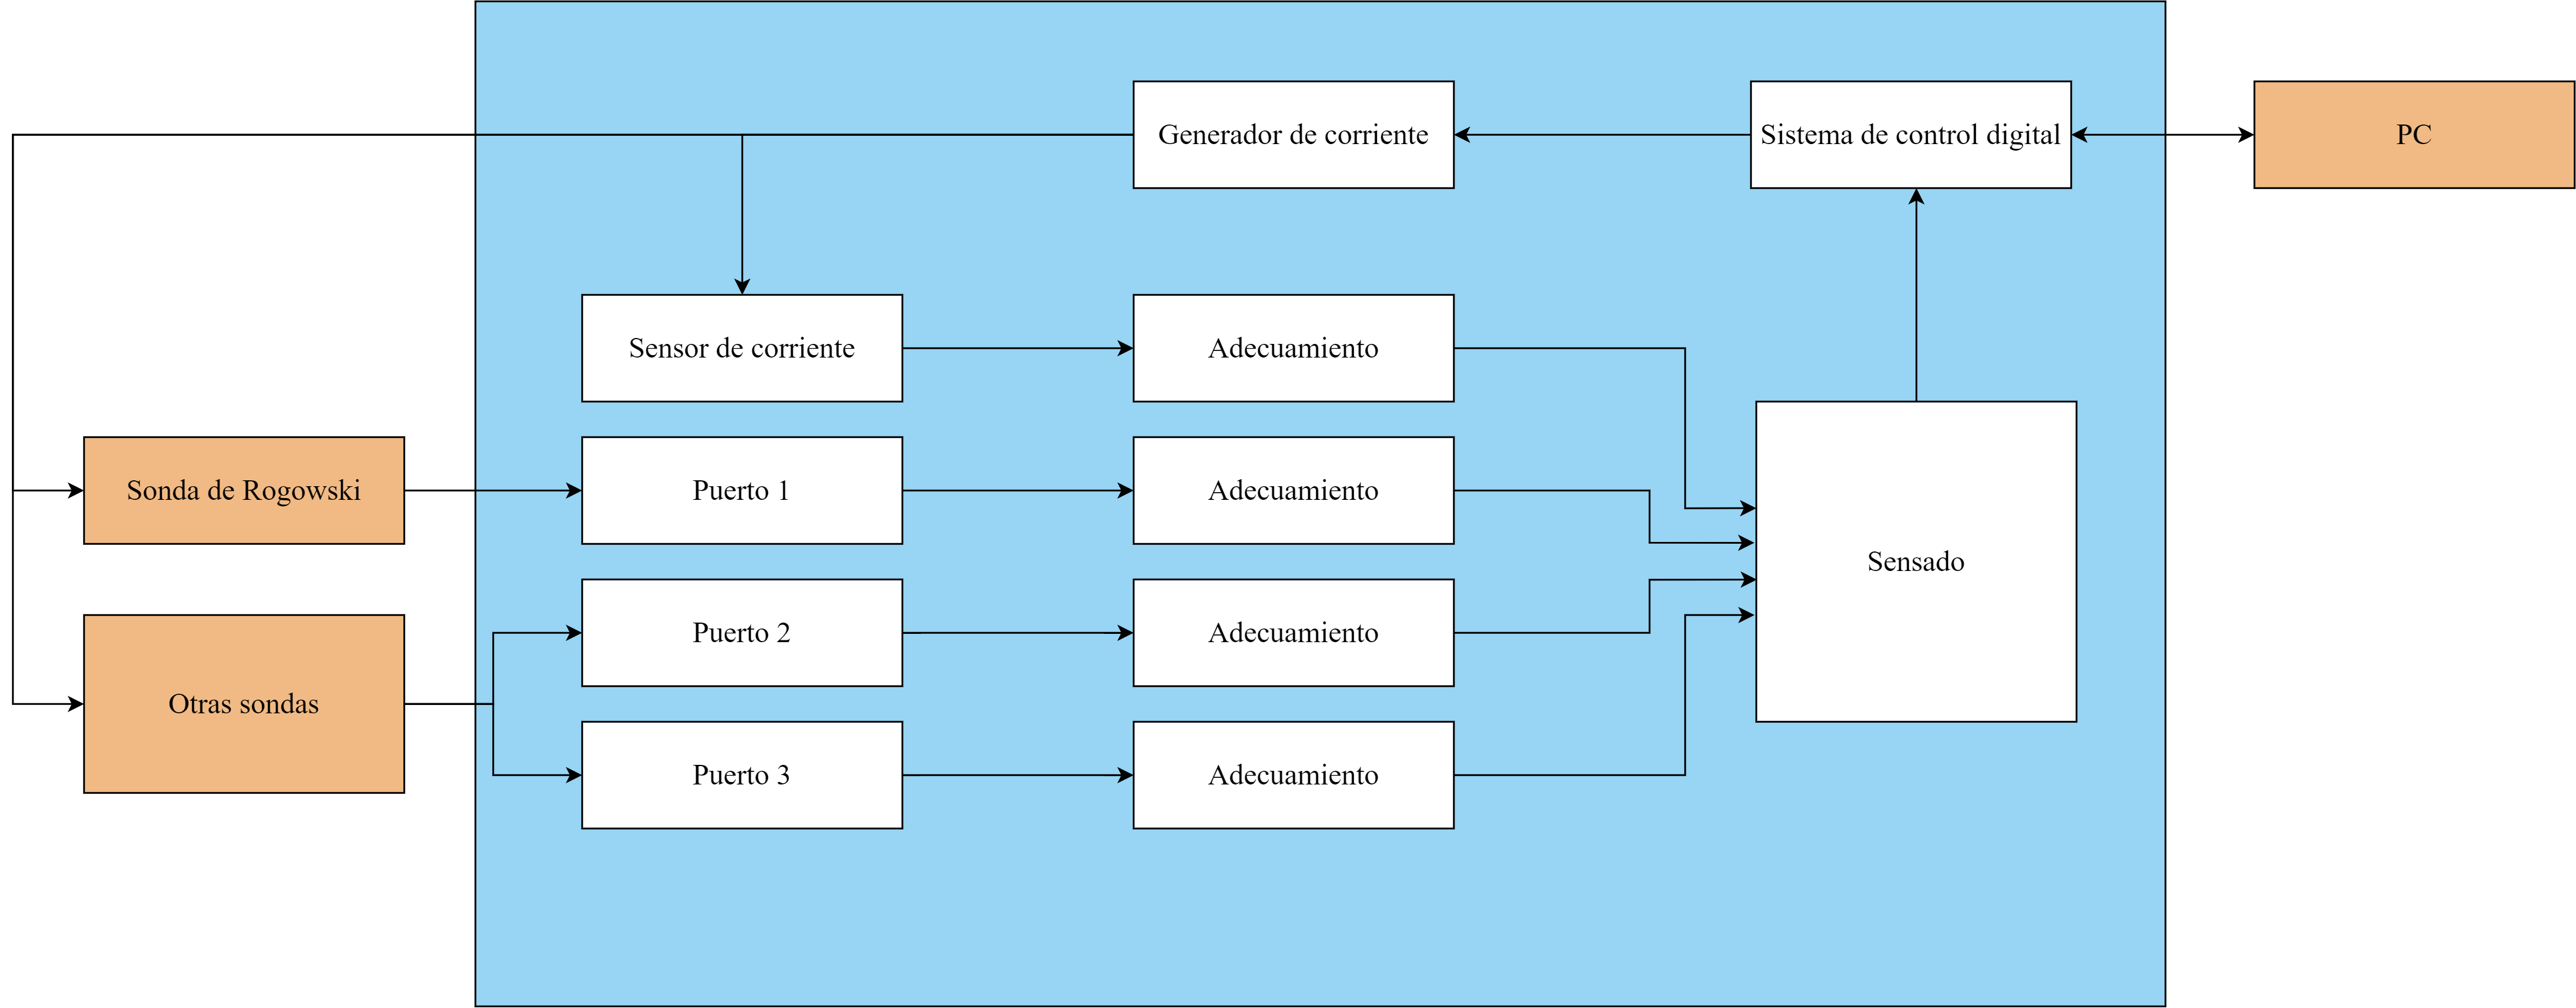
\includegraphics[width=\textwidth]{diagrams/bloques-general.png}
    \caption{Diagrama en bloques general del dispositivo}
    \label{fig:bloques-general}
  \end{figure}

  Este instrumento permitirá generar corrientes que alimenten a las sondas a calibrar o caracterizar. Luego, las mediciones tomadas por estas sondas serán introducidas al instrumento para su posterior análisis.

  Los resultados de estas calibraciones o caracterizaciones, serán mostradas a través de una interfaz gráfica en una PC, a la que estará conectado el instrumento. Esta permitirá controlar todas las funciones del mismo.


  %% ----------------------------------------------------------------
  \section{Especificaciones funcionales}
  %% ----------------------------------------------------------------

  %% ----------------------------------------------------------------
  \subsection{RF01: Generación y adquisición de corriente}
  %% ----------------------------------------------------------------
  El instrumento deberá poder generar corriente alterna, que será posteriormente adquirida para ser controlada a lazo cerrado por un sistema de control digital. Se podrán generar las siguientes formas de onda:

  \begin{itemize}
    \item Senoidal
    \item Cuadrada
    \item Triangular
    \item Diente de sierra
    \item Otras personalizadas por el usuario
  \end{itemize}

  La corriente alterna máxima que se permitirá es de \SI{10}{A_{rms}}. La frecuencia máxima permitida será de \SI{2000}{Hz}, siendo esta el 40º armónico de la frecuencia de línea de energía en Argentina.

  Esta corriente generada deberá poder ser medida por sondas de corriente externas, las cuales se conectarán al instrumento y permitirán la adquisición de estas mediciones. El dispositivo contará así con tres puertos para esta tarea, uno de los cuales será exclusivo para sondas de Rogowski y los demás genéricos para otras sondas.

  Luego del puerto de conexión de las sondas, se agregará una etapa de adecuamiento, de manera de eliminar ruido y ajustar la ganancia de las señales adquiridas para la etapa posterior de sensado. Finalmente las mediciones serán introducidas al sistema de control digital, el cual realizará un procesamiento de los datos, produciendo la siguiente información:

    \begin{itemize}
      \item Amplitud RMS
      \item Amplitud RMS de armónicos, fundamental y continua
      \item Distorsión total de la forma de onda (TWD)
    \end{itemize}

  %% ----------------------------------------------------------------
  \subsection{RF02: Sistema de control gráfico y gestión de ensayos}
  %% ----------------------------------------------------------------
  El dispositivo deberá ser capaz de conectarse a una PC que utilice el sistema operativo Windows. En la misma correrá una interfaz gráfica que permitirá darle instrucciones al instrumento, así como también reportar información proveniente del mismo.

  En la \autoref{fig:gui} se puede observar un esquema a modo de guía para el diseño de la interfaz gráfica.

  \begin{figure}[!htbp]
    \centering
    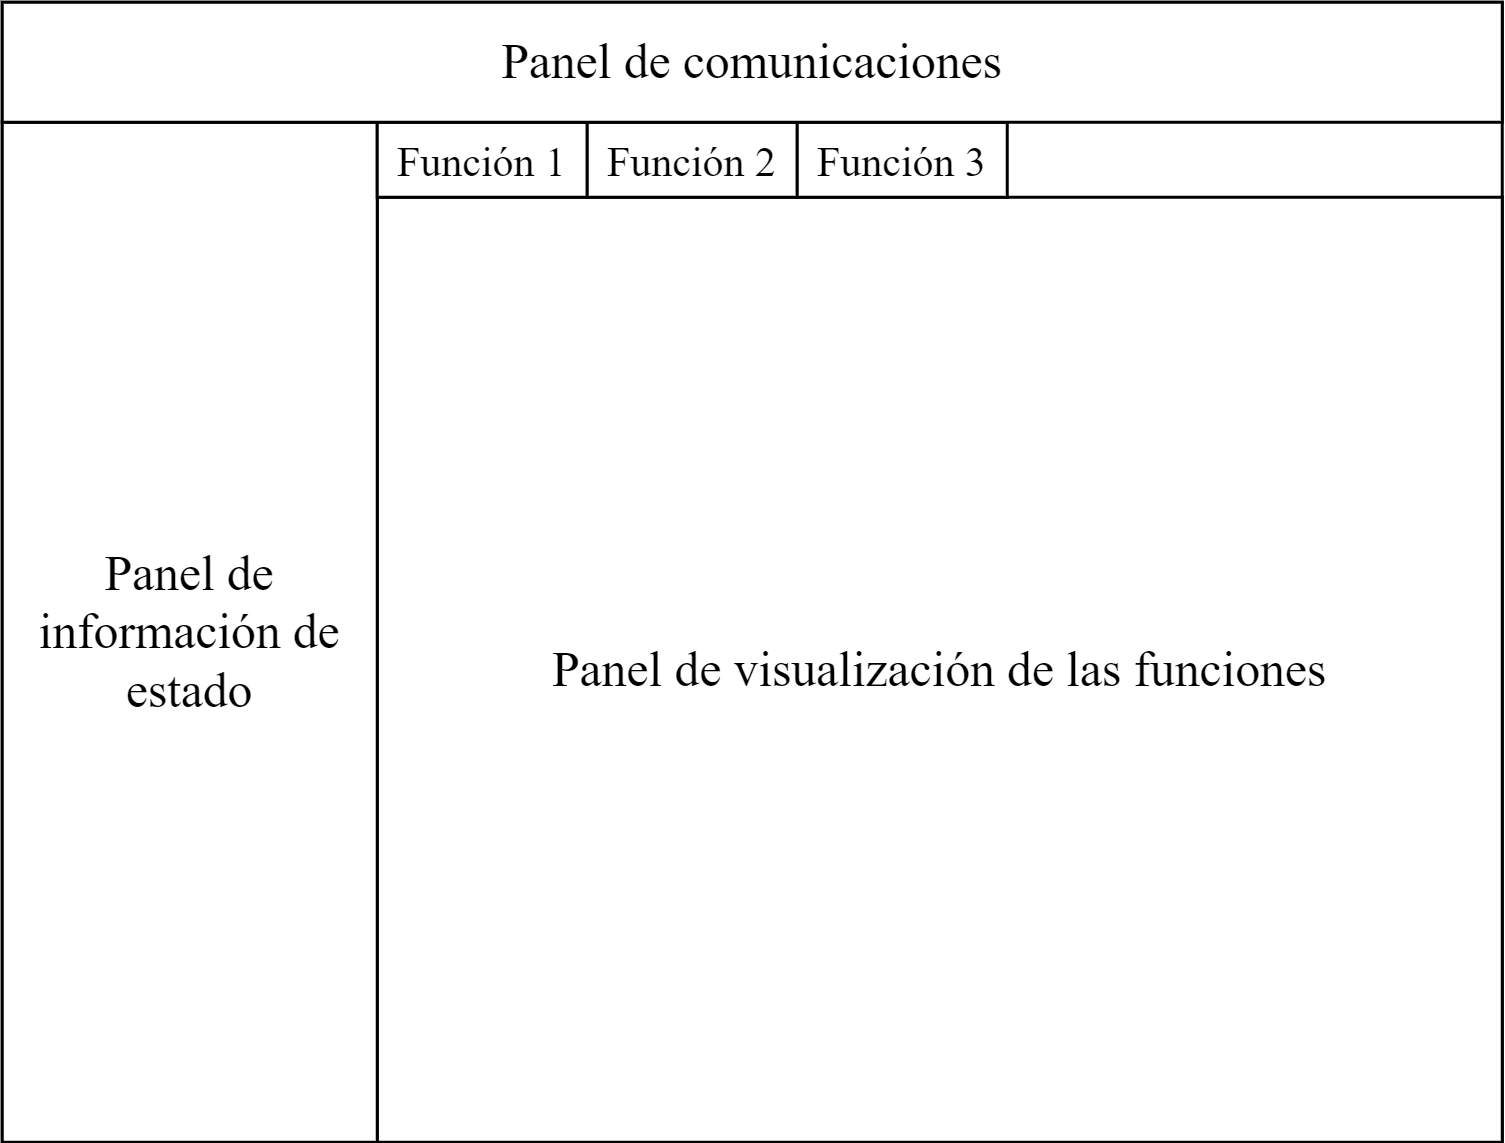
\includegraphics[width=0.8\textwidth]{diagrams/gui.png}
    \caption{Esquema de la interfaz gráfica}
    \label{fig:gui}
  \end{figure}

  En el ``Panel de comunicaciones'' se deberá colocar todos los elementos referidos a las comunicaciones. Entre ellos el estado de conexión, la selección del puerto de la PC al que se conectó el instrumento y botones para conectar y desconectar.

  En el ``Panel de información de estado'' se deberá colocar todos los elementos relacionados con la configuración de la interfaz gráfica y del instrumento. Se mostrará tanto la configuración existente en ambos y se podrá modificar desde el mismo panel.

  En el ``Panel de visualización de las funciones'' se colocarán todos los elementos correspondiente a las funciones. En la \autoref{fig:gui} se observan los botones de cambio de función, que modificarán el panel de acuerdo a la función que se encuentre seleccionada.

  El instrumento deberá ser capaz de realizar ensayos automatizados. El usuario deberá poder introducir los parámetros necesarios del ensayo en la interfaz gráfica en la PC, para que al finalizar el mismo, genere un reporte de caracterización de las sondas conectadas.

  Los ensayos automatizados que se deberá proveer, serán de dos tipos:

    \begin{itemize}
      \item Ensayo de respuesta en frecuencia
      \item Ensayo de respuesta en frecuencia con control de máximo TWD
    \end{itemize}

  En ambos ensayos los parámetros a ingresar serán:

    \begin{itemize}
      \item Amplitud RMS
      \item Frecuencia inicial
      \item Frecuencia final
      \item Frecuencia de paso
    \end{itemize}

  Agregándose para el segundo ensayo el siguiente parámetro:

    \begin{itemize}
      \item Máximo TWD permitido
    \end{itemize}

  Se deberá además soportar un modo ``generador'' en el cual el usuario pueda utilizar el instrumento en modo libre, permitiéndosele ingresar los siguientes parámetros:

    \begin{itemize}
      \item Amplitud RMS
      \item Frecuencia
      \item Forma de onda
    \end{itemize}


%% ----------------------------------------------------------------
\section{Requerimientos no funcionales}
%% ----------------------------------------------------------------

  %% ----------------------------------------------------------------
  \subsection{RNF01: Generación de informes en PDF o JPG}
  %% ----------------------------------------------------------------
  Los informes mostrados en la interfaz gráfica deberán poder ser guardados en formato PDF o JPG, para su posterior uso.

  Se le deberá mostrar al usuario una ventana en la que podrá seleccionar el nombre del archivo a guardar y su ubicación. Se guardará la misma información que la mostrada en pantalla en el informe.

  %% ----------------------------------------------------------------
  \subsection{RNF02: Guardado de datos en formato CSV}
  %% ----------------------------------------------------------------
  Los datos generados en los reportes deberán poder ser guardados en formato CSV (\emph{comma-separated values}). Esto permitirá al usuario acceder a los datos ``crudos'' y realizar así, en caso de necesitarlo, un procesado adicional.

  Los datos serán guardados con el siguiente formato:

  \begin{table}[!hbtp]
    \centering
      \begin{tabular}{|c|c|c|l|l|}
      \hline
      \rowcolor[HTML]{C0C0C0}
      Frequency & Channel & Irms & TWD & Harmonic $n$ \\ \hline
                &         &      &     &              \\ \hline
      \end{tabular}
  \end{table}

  %% ----------------------------------------------------------------
  \subsection{RNF03: Registro de eventos}
  %% ----------------------------------------------------------------
  La interfaz gráfica deberá tener implementado un registro de eventos o \emph{logging} que permita al usuario obtener información de los distintos sucesos que ocurran en el dispositivo.

  Se tendrán distintos niveles de registro, que se reportarán y podrán ser filtrados por el usuario:

  \begin{itemize}
    \item \emph{Critical}: sucesos que fuercen a un apagado del instrumento
    \item \emph{Error}: sucesos que causen fallas en la operación del instrumento, pero no en sí mismo
    \item \emph{Warning}: sucesos que puedan, pero no necesariamente lo hagan, causar fallas en el sistema
    \item \emph{Info}: sucesos de información
    \item \emph{Debug}: sucesos de diagnóstico
  \end{itemize}

  Se deberá agregar además un modo en el que el usuario podrá observar los datos ``crudos'' transmitidos entre el instrumento y la PC.

\end{document}
